%-------------------------------------------------------------------------------
% seq66_sessions
%-------------------------------------------------------------------------------
%
% \file        seq66_sessions.tex
% \library     Documents
% \author      Chris Ahlstrom
% \date        2020-10-03
% \update      2020-10-09
% \version     $Revision$
% \license     $XPC_GPL_LICENSE$
%
%  Provides a discussion of how Seq66 supports session management, specifically
%  the Non Session Manager.
%
%-------------------------------------------------------------------------------

\section{Seq66 Session Management}
\label{sec:sessions}

   \textsl{Seq66} supports session management in three ways:

   \begin{enumber}
      \item \textbf{Non Session Manager}
      \item \textbf{Signals}
      \item \textbf{LASH}
   \end{enumber}

%  See \sectionref{subsec:seq66_rc_file_midi_control},

\subsection{Seq66 Session Management / NSM}
\label{subsec:sessions_nsm}

   \index{sessions!nsm}
   MORE TO COME.  NSM support is well underway, but still in progress

\subsubsection{Seq66 Session Management / NSM / First Run Before Using NSM}
\label{subsec:sessions_nsm_before_using_nsm}

   It is important, after installing \textsl{Seq66}, to run it normally. This
   action creates the default configuration files in
   \texttt{/home/user/.config/seq66}.

\begin{verbatim}
   nsm $ qseq66 
   [No 'rc' file, will create: qseq66.rc/ctrl/midi/mutes/drums/playlist]
   [No 'usr' file, will create: /home/user/.config/seq66/qseq66.usr]
   [File exists: /home/user/.config/seq66/qseq66.rc]
   [Saving initial config files to session directory!]
   [Writing 'rc': /home/user/.config/seq66/qseq66.rc]
   [Writing 'ctrl': /home/user/.config/seq66/qseq66.ctrl]
   [Writing 'mutes': /home/user/.config/seq66/qseq66.mutes]
   [Writing 'usr': /home/user/.config/seq66/qseq66.usr]
\end{verbatim}

   The \texttt{qseq66.usr} file can then be edited to allow \textsl{Seq66} to
   use NSM.  Look for the following lines in that file:

\begin{verbatim}
   [user-session]
   session = none
\end{verbatim}

   Change the "session" line to

\begin{verbatim}
   session = nsm
\end{verbatim}

   Then we are ready to run the Non Session Manager, as described in the next
   section.

\subsubsection{Seq66 Session Management / NSM / First Run}
\label{subsec:sessions_nsm}

   Now that we have the initial configuration, we want to run \textsl{Seq66}
   under NSM and create a configuration in the NSM sessions directory.

\begin{verbatim}
   $ non-session-manager
   [non-session-manager] Starting daemon...
   [nsmd] Session root is: /home/chris/NSM Sessions
   NSM_URL=osc.udp://mlsasus.mls:19625/
   [nsmd] Listing sessions
\end{verbatim}

   The NSM user-interface that comes up is empty at first.  So we now create a
   session by clicking the NSM \textsl{New} button, and entering a session name
   (e.g. "Seq66") in the prompt that comes up.  We see, in the console window,
   a couple of
   "/nsm/server/new" \textsl{OSC} messages about the creation of the session.

\begin{verbatim}
   [non-session-manager] Sending new for: Seq66
   [nsmd] Creating new session "Seq66"
   [non-session-manager] /nsm/server/new says Created.
   [non-session-manager] /nsm/server/new says Session created
\end{verbatim}

   Next, we click the \textsl{Add Client to Session}, and, since
   \texttt{qseq66} has been installed, it is in the "PATH" and its executable
   name can be entered simply: "qseq66".



\subsubsection{Seq66 Session Management / User Interface}
\label{subsubsec:sessions_ui}

   \index{sessions!ui}
   This section describes the \textsl{Session} tab in the main
   \textsl{Seq66} window.

   MORE TO COME.

\subsection{Seq66 Session Management / Signals}
\label{subsec:sessions_signals}

   \index{sessions!signals}
   By default, the basic form of session management in
   \textsl{Seq66} occurs by signals.  A
   session manager can start \textsl{Seq66}, and it can tell \textsl{Seq66} to
   save or stop.  Starting is done by a system call to spawn the application.
   The save and stop actions are supported by sending the following signals to
   the application:

   \begin{itemize}
      \item \texttt{SIGINT}.  This signal stops \textsl{Seq66}. It corresponds
         to using \texttt{Ctrl-C} from the command-line to stop \textsl{Seq66}.
         This signal should work for both the graphical and command-line
         application.  As \textsl{Seq66} shuts down, it does its normal saving
         of the current state of the configuration.
      \item \texttt{SIGTERM}.  This signal also stops \textsl{Seq66}.  It can
         be sent by an application to exit \textsl{Seq66}.
      \item \texttt{SIGUSR1}.  This signal tells \textsl{Seq66} to save.  This
         action will save the current MIDI file.
   \end{itemize}

   One application that can control \textsl{Seq66} is \textsl{nsm-proxy}:

      \url{https://non.tuxfamily.org/wiki/nsm-proxy}

   NSM-Proxy is a simple NSM client for wrapping non-NSM capable programs. It
   enables the use of programs supporting LADISH Level 0 and 1, and programs
   which accept their configuration via command-line arguments.  There is a
   command-line version and a graphical version.

   MORE TO COME on how to use nsm-proxy.

\subsection{Seq66 Session Management / LASH}
\label{subsec:sessions_lash}

   \index{sessions!lash}
   MORE TO COME.  LASH support has not yet been fully reimplemented and retested.


%\begin{figure}[H]
%   \centering 
%   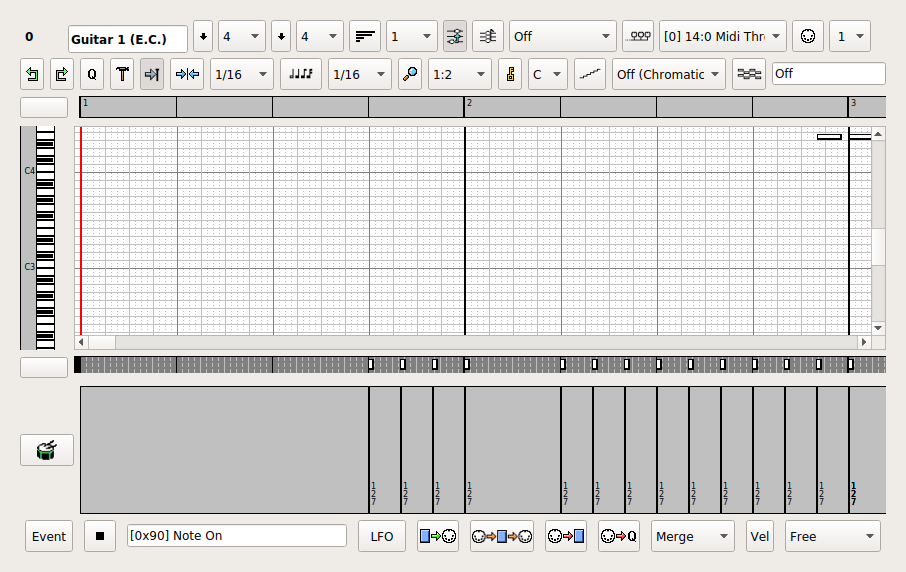
\includegraphics[scale=0.65]{roll.png}
%   \caption*{Qt 5 Playlist Tab}
%\end{figure}


%-------------------------------------------------------------------------------
% vim: ts=3 sw=3 et ft=tex
%-------------------------------------------------------------------------------
